\documentclass{article}

\usepackage{fancyhdr}
\usepackage{extramarks}
\usepackage{amsmath,mathrsfs,amssymb}
\usepackage{amsthm}
\usepackage{amsfonts}
\usepackage{tikz}
\usepackage[plain]{algorithm}
\usepackage{algpseudocode}
\usepackage[]{mcode}
\usepackage{graphicx}
\usepackage{pgfplots}
\usepackage{xfrac,siunitx}
\usepackage{gensymb}
\usepackage{caption}
\usepackage{epstopdf}

\usetikzlibrary{automata,positioning}
\usetikzlibrary{calc}
\usetikzlibrary{shapes,arrows}

%
% Basic Document Settings
%

\topmargin=-0.45in
\evensidemargin=0in
\oddsidemargin=0in
\textwidth=6.5in
\textheight=9.0in
\headsep=0.25in

\linespread{1.1}

\pagestyle{fancy}
\lhead{\hmwkAuthorName}
\chead{\hmwkClass\ (\hmwkClassInstructor\ \hmwkClassTime): \hmwkTitle}
\rhead{\firstxmark}
\lfoot{\lastxmark}
\cfoot{\thepage}

\renewcommand\headrulewidth{0.4pt}
\renewcommand\footrulewidth{0.4pt}

\setlength\parindent{0pt}

%
% Create Problem Sections
%

\newcommand{\enterProblemHeader}[1]{
    \nobreak\extramarks{}{Problem \arabic{#1} continued on next page\ldots}\nobreak{}
    \nobreak\extramarks{Problem \arabic{#1} (continued)}{Problem \arabic{#1} continued on next page\ldots}\nobreak{}
}

\newcommand{\exitProblemHeader}[1]{
    \nobreak\extramarks{Problem \arabic{#1} (continued)}{Problem \arabic{#1} continued on next page\ldots}\nobreak{}
    \stepcounter{#1}
    \nobreak\extramarks{Problem \arabic{#1}}{}\nobreak{}
}

\setcounter{secnumdepth}{0}
\newcounter{partCounter}
\newcounter{homeworkProblemCounter}
\setcounter{homeworkProblemCounter}{1}
\nobreak\extramarks{Problem \arabic{homeworkProblemCounter}}{}\nobreak{}

%
% Homework Problem Environment
%
% This environment takes an optional argument. When given, it will adjust the
% problem counter. This is useful for when the problems given for your
% assignment aren't sequential. See the last 3 problems of this template for an
% example.
%
\newenvironment{homeworkProblem}[1][-1]{
    \ifnum#1>0
        \setcounter{homeworkProblemCounter}{#1}
    \fi
    \section{Problem \arabic{homeworkProblemCounter}}
    \setcounter{partCounter}{1}
    \enterProblemHeader{homeworkProblemCounter}
}{
    \exitProblemHeader{homeworkProblemCounter}
}

%
% Homework Details
%   - Title
%   - Due date
%   - Class
%   - Section/Time
%   - Instructor
%   - Author
%

\newcommand{\hmwkTitle}{Tutorial\ 3}
\newcommand{\hmwkDueDate}{August 09, 2016}
\newcommand{\hmwkClass}{Control Engineering}
\newcommand{\hmwkClassTime}{}
\newcommand{\hmwkClassInstructor}{Professor Friso De Boer}
\newcommand{\hmwkAuthorName}{S.Reynolds (262538)}

%
% Title Page
%

\title{
    \vspace{2in}
    \textmd{\textbf{\hmwkClass:\ \hmwkTitle}}\\
    \normalsize\vspace{0.1in}\small{Due\ on\ \hmwkDueDate\ at 3:00pm}\\
    \vspace{0.1in}\large{\textit{\hmwkClassInstructor\ \hmwkClassTime}}
    \vspace{3in}
}

\author{\textbf{\hmwkAuthorName}}
\date{}

\renewcommand{\part}[1]{\textbf{\large Part \Alph{partCounter}}\stepcounter{partCounter}\\}

%
% Various Helper Commands
%

% Useful for algorithms
\newcommand{\alg}[1]{\textsc{\bfseries \footnotesize #1}}

% For derivatives
\newcommand{\deriv}[1]{\frac{\mathrm{d}}{\mathrm{d}x} (#1)}

% For partial derivatives
\newcommand{\pderiv}[2]{\frac{\partial}{\partial #1} (#2)}

% Integral dx
\newcommand{\dx}{\mathrm{d}x}

% Alias for the Solution section header
\newcommand{\solution}{\textbf{\large Solution}}

% Probability commands: Expectation, Variance, Covariance, Bias
\newcommand{\E}{\mathrm{E}}
\newcommand{\Var}{\mathrm{Var}}
\newcommand{\Cov}{\mathrm{Cov}}
\newcommand{\Bias}{\mathrm{Bias}}

\DeclareMathOperator{\sinc}{sinc}

\begin{document}

\maketitle

\pagebreak

%%%%%%%%%%%%%%%%%%%%%%%%%%%%%%%%%%%%%%%%%%%%%%%%%%%%%%%%%%%%%%%%%%%%%%%%%%%%%%%%%%%%%%%%%%%%%%%%%%%%%%%%%%%%%%%%%%%%%%
% Question 2.1
%%%%%%%%%%%%%%%%%%%%%%%%%%%%%%%%%%%%%%%%%%%%%%%%%%%%%%%%%%%%%%%%%%%%%%%%%%%%%%%%%%%%%%%%%%%%%%%%%%%%%%%%%%%%%%%%%%%%%% 


    \textbf{Question 3.1}\\
    
    We note that from the previous rocket control tutorial that $H(s) = 1$, and that the open loop controller and plant form the system $G(s)$, that is:
    \begin{align}
	    G(s) = G_C(s) \cdot G_P(s) = K \cdot \frac{s + 1}{s^2}
    \end{align}
    
	By inspection, the controlled system has zeros $z_1 = -1$, and poles $p_1 = 0$ and $p_2 = 0$ (that is the pole is repeated). The plotted poles and zeros can be seen in Figure 1.
	
	\begin{figure}[h]
		\centering
		\begin{tikzpicture}
		\begin{axis}[
		scale=1.4,
		xmin=-6,
		xmax=1,
		ymin=-2,
		ymax=2,
		axis lines = middle,
		xlabel = $Re$,
		ylabel = {$Im$},
		xtick = {-5,...,0},
		ytick = {-2,...,2},
		axis equal
		]
		
		\addplot[blue,mark=o,mark size=3] coordinates {(-1,0)};
		\addplot[red,mark=x,mark size=3] coordinates {(0,0)};
		\addplot[red,mark=+,mark size=3] coordinates {(0,0)};
		\end{axis}
		
		\end{tikzpicture}
		\caption{Poles and zeros of the open loop system}
	\end{figure}
	
%%%%%%%%%%%%%%%%%%%%%%%%%%%%%%%%%%%%%%%%%%%%%%%%%%%%%%%%%%%%%%%%%%%%%%%%%%%%%%%%%%%%%%%%%%%%%%%%%%%%%%%%%%%%%%%%%%%%%%
% Question 2.2
%%%%%%%%%%%%%%%%%%%%%%%%%%%%%%%%%%%%%%%%%%%%%%%%%%%%%%%%%%%%%%%%%%%%%%%%%%%%%%%%%%%%%%%%%%%%%%%%%%%%%%%%%%%%%%%%%%%%%%

 
    \textbf{Question 2.2}\\
    
    To find the root locus on the real axis, we need to consider the angle of the open loop system in the intervals that the poles and zeros make. That is we need to consider the equation (1) for the intervals $s > 0$, $-1 < s < 0$, and $s < -1$. The equation is as follows:
    \begin{align}
	    \angle G(s)H(s) = \angle (K \cdot (s+1)) - 2 \cdot \angle s =  \angle K + \angle (s+1) - 2 \cdot \angle s
    \end{align}
	
	Hence, we make the following observations using equation (2):
	\begin{align*}
		\angle G(s)H(s)_{s \in (0,\infty)} &= 0\si{\degree} + 0\si{\degree} - 2 \cdot 0\si{\degree} = 0\si{\degree} \neq 180\si{\degree}(2k + 1)\\
		\angle G(s)H(s)_{s \in (-1,0]} &= 0\si{\degree} + 0\si{\degree} - 2 \cdot 180\si{\degree} = -360\si{\degree} \neq 180\si{\degree}(2k + 1)\\
		\angle G(s)H(s)_{s \in (-\infty,-1]} &= 0\si{\degree} + 180\si{\degree} - 2 \cdot 180\si{\degree} = -180\si{\degree} = 180\si{\degree}(2k + 1)
	\end{align*}
	
	Hence, the root locus on the real axis occurs on the real axis for the interval $s \in (-\infty, -1)$. The plot can be seen in Figure 2.
	
	\begin{figure}[h]
		\centering
		\begin{tikzpicture}
		\begin{axis}[
		scale=1.4,
		xmin=-6,
		xmax=1,
		ymin=-2,
		ymax=2,
		axis lines = middle,
		xlabel = $Re$,
		ylabel = {$Im$},
		xtick = {-5,...,0},
		ytick = {-2,...,2},
		axis equal
		]
		
		\addplot[blue,mark=o,mark size=3] coordinates {(-1,0)};
		\addplot[red,mark=x,mark size=3] coordinates {(0,0)};
		\addplot[red,mark=+,mark size=3] coordinates {(0,0)};
		\draw[green, ->, thick] (axis cs:-1,0) -- (axis cs:-5,0);
		\end{axis}
		
		\end{tikzpicture}
		\caption{Plot of the part of the root locus which runs along the real axis}
	\end{figure}
	
%%%%%%%%%%%%%%%%%%%%%%%%%%%%%%%%%%%%%%%%%%%%%%%%%%%%%%%%%%%%%%%%%%%%%%%%%%%%%%%%%%%%%%%%%%%%%%%%%%%%%%%%%%%%%%%%%%%%%%
% Question 2.3
%%%%%%%%%%%%%%%%%%%%%%%%%%%%%%%%%%%%%%%%%%%%%%%%%%%%%%%%%%%%%%%%%%%%%%%%%%%%%%%%%%%%%%%%%%%%%%%%%%%%%%%%%%%%%%%%%%%%%%

	\newpage
    \textbf{Question 2.3}\\
    
    If the number of poles and zeros in equation (1) are $n$ and $m$, respectively, then using equation (3) we can find the angle at which the root locus asymptote departs the real axis, with formula shown below:
    \begin{align}
	    \theta = \frac{180\si{\degree}(2k + 1)}{n - m}
    \end{align}
    
	We note that there will only be a single asymptote, since, $n - m = 2 - 1 = 1$ and its angle of departure from the real axis is:
	\begin{align*}
		\theta = \frac{180\si{\degree}(2k+1)}{2 - 1} = 180\si{\degree}
	\end{align*}
	
	The centroid is the point on the real axis at which the asymptotes intersect. Since we only have a single asymptote, this value does not yield much insight which sketching the root locus. Nonetheless, the centroid is given by:
	\begin{align*}
		\sigma_A = \frac{\sum_{i = 1}^{2} p_i - \sum_{j = 1}^{1} z_j}{n - m} = \frac{0 + 0 - - 1}{2 - 1} = 1
	\end{align*}
	
	The asymptote runs along the real axis towards $-\infty$, hence, this would not be visible on the plot.\\
%%%%%%%%%%%%%%%%%%%%%%%%%%%%%%%%%%%%%%%%%%%%%%%%%%%%%%%%%%%%%%%%%%%%%%%%%%%%%%%%%%%%%%%%%%%%%%%%%%%%%%%%%%%%%%%%%%%%%%
% Question 2.4
%%%%%%%%%%%%%%%%%%%%%%%%%%%%%%%%%%%%%%%%%%%%%%%%%%%%%%%%%%%%%%%%%%%%%%%%%%%%%%%%%%%%%%%%%%%%%%%%%%%%%%%%%%%%%%%%%%%%%%


   \textbf{Question 2.4}\\
    
   To find the break in and break out points, we first need to write the characteristic polynomial\\ $1 + G(s)H(s) = 0$ in the form $B(s) + K \cdot A(s) = 0$.
   \begin{align}
	   1 + G(s)H(s) = B(s) + K \cdot A(s) = 1 + K \cdot \frac{s + 1}{s^2}
   \end{align}
   
   From equation (4), we see that $B(s) = 1$, and $A(s) = \frac{s + 1}{s^2}$. Rearranging $B(s) + K \cdot A(s) = 0$, we get that $K = -\frac{B(s)}{A(s)}$. The break in and break out points occur at the points $s$, when $\frac{dK}{ds} = 0$. Hence, we get that:
   \begin{align*}
	   \frac{dK}{ds} = - \frac{B'(s)A(s) - B(s)A'(s)}{[A(s)]^2} = - \frac{0 \cdot A(s) - (-s^{-2} - 2s^{-3})}{[\frac{s+1}{s^2}]^2} = - \frac{s^4(s^{-2} + 2s^{-3})}{(s+1)^2}
   \end{align*}
   
   Hence, if we set $\frac{dK}{ds} = 0$, then we find that:
   \begin{align}
	   s^4(s^{-2} + 2s^{-3}) = 0
   \end{align}
   
   Solving the part of equation (5) which is in brackets, we get that:
   \begin{align*}
	   s^{-2} + 2s^{-3} &= 0\\
	   s + 2 &= 0\\
	   s &= -2
   \end{align*}
   
   Hence, the break out point occurs at $s = 0$, and we find that the break in point occurs at $s = -2$.\\
%%%%%%%%%%%%%%%%%%%%%%%%%%%%%%%%%%%%%%%%%%%%%%%%%%%%%%%%%%%%%%%%%%%%%%%%%%%%%%%%%%%%%%%%%%%%%%%%%%%%%%%%%%%%%%%%%%%%%%
% Question 2.5
%%%%%%%%%%%%%%%%%%%%%%%%%%%%%%%%%%%%%%%%%%%%%%%%%%%%%%%%%%%%%%%%%%%%%%%%%%%%%%%%%%%%%%%%%%%%%%%%%%%%%%%%%%%%%%%%%%%%%%
	
   \textbf{Question 2.5}\\
	
   Step 5 calculates the angle of departure of complex poles, however, this step can be ignored because there are no complex poles. Step 6 can be ignored since none of the poles will cross the imaginary axis - one pole will match up with the zero and the other will move off toward negative infinity.\\
	
%%%%%%%%%%%%%%%%%%%%%%%%%%%%%%%%%%%%%%%%%%%%%%%%%%%%%%%%%%%%%%%%%%%%%%%%%%%%%%%%%%%%%%%%%%%%%%%%%%%%%%%%%%%%%%%%%%%%%%
% Question 2.6
%%%%%%%%%%%%%%%%%%%%%%%%%%%%%%%%%%%%%%%%%%%%%%%%%%%%%%%%%%%%%%%%%%%%%%%%%%%%%%%%%%%%%%%%%%%%%%%%%%%%%%%%%%%%%%%%%%%%%%

	\textbf{Question 2.6}\\
	
	The characteristic equation $1 + G(s)H(s) = 0$ can be written in two different forms. The first form is:  and 
	\begin{align}
		K = - \frac{s^2}{s+1}
	\end{align}
	
	And the second form is:
	\begin{align}
		s^2 + Ks + K = 0
	\end{align}
	
	Now in order to plot the root locus, we need to choose some test points in the $s$-plane about the origin. The first point is $s = 5$. Hence, from equation (6) we get that:
	\begin{align*}
		K 	&= -\frac{(-5)^2}{1-5}\\
			&= \frac{-25}{-4}\\
			&= 6.25
	\end{align*}
	
	Given that $K = 6.25$, we can find the other pole using equation (7):
	\begin{align*}
		s^2 + 6.25s + 6.25 = 0\\
		\therefore \quad s=-5, \quad s=-1.25
	\end{align*}
	
	The second test point is $s = -1 + j$, which using equation (6), gives us the following solution:
	\begin{align*}
		K 	&= \frac{-(-1+j)^2}{-1 + j + 1} \cdot \frac{j}{j}\\
			&= j \cdot (-1 + j)^2\\
			&= -2 \cdot j^2\\
			&= 2
	\end{align*}
	
	Given that $K = 2$, we can find the other pole using equation (7):
	\begin{align*}
		s^2 + 2s + 2 = 0\\
		\therefore \quad s = -1 \pm j
	\end{align*}
	
	\newpage
	
	A sketch of the root locus plot, done using pgf plots, can be seen in Figure 3.
	\begin{figure}[h]
		\centering
		\begin{tikzpicture}
		\begin{axis}[
		scale=1.4,
		xmin=-6,
		xmax=1,
		ymin=-2,
		ymax=2,
		axis lines = middle,
		xlabel = $Re$,
		ylabel = {$Im$},
		xtick = {-5,...,0},
		ytick = {-2,...,2},
		axis equal
		]
		
		\addplot[blue,mark=o,mark size=3] coordinates {(-1,0)};
		\addplot[red,mark=x,mark size=3] coordinates {(0,0)};
		\addplot[red,mark=+,mark size=3] coordinates {(0,0)};
		\addplot[domain=-2:0,green,thick] {(1-(x+1)^2)^0.5};
		\draw[green, ->,thick] (axis cs:-2,0) -- (axis cs:-1,0);
		\addplot[domain=-2:0,purple,thick] {-(1-(x+1)^2)^0.5};
		\draw[purple, <-,thick] (axis cs:-4,0) -- (axis cs:-2,0);
		\end{axis}
		
		\end{tikzpicture}
		\caption{Plot of the root locus}
	\end{figure}
	
	\newpage
	
%%%%%%%%%%%%%%%%%%%%%%%%%%%%%%%%%%%%%%%%%%%%%%%%%%%%%%%%%%%%%%%%%%%%%%%%%%%%%%%%%%%%%%%%%%%%%%%%%%%%%%%%%%%%%%%%%%%%%%
% Question 2.7
%%%%%%%%%%%%%%%%%%%%%%%%%%%%%%%%%%%%%%%%%%%%%%%%%%%%%%%%%%%%%%%%%%%%%%%%%%%%%%%%%%%%%%%%%%%%%%%%%%%%%%%%%%%%%%%%%%%%%%

	\textbf{Question 2.7}\\
	
	Pole locations were found for various values of the gain $K$. The values are as follows:
	\begin{itemize}
		\item For $K = 1$, the characteristic equation is given by $s^2 + s + 1 = 0$, which has poles $s = -0.5 \pm j0.866$.
		\item For $K = 2$, the characteristic equation is given by $s^2 + 2s + 2 = 0$, which has poles $s = -1 \pm j$.
		\item For $K = 3$, the characteristic equation is given by $s^2 + 3s + 3 = 0$, which has poles $s = -1.5 \pm j0.866$.
		\item For $K = 4$, the characteristic equation is given by $s^2 + 5s + 5 = 0$, which has poles $s = -6.25$, and $s = -1.25$.
	\end{itemize}
	
	The pole values for different values of $K$ calculated above are shown in Figure 4 below.\\
	
	\begin{figure}[h]
		\centering
		\begin{tikzpicture}
		\begin{axis}[
		scale=1.4,
		xmin=-6,
		xmax=1,
		ymin=-2,
		ymax=2,
		axis lines = middle,
		xlabel = $Re$,
		ylabel = {$Im$},
		xtick = {-5,...,0},
		ytick = {-2,...,2},
		axis equal
		]
		
		\addplot[blue,mark=o,mark size=3] coordinates {(-1,0)};
		\addplot[red,mark=x,mark size=3] coordinates {(0,0)};
		\addplot[red,mark=+,mark size=3] coordinates {(0,0)};
		\addplot[domain=-2:0,green,thick] {(1-(x+1)^2)^0.5};
		\draw[green, ->,thick] (axis cs:-2,0) -- (axis cs:-1,0);
		\addplot[domain=-2:0,purple,thick] {-(1-(x+1)^2)^0.5};
		\draw[purple, <-,thick] (axis cs:-4,0) -- (axis cs:-2,0);
		
		\addplot[blue,mark=*,mark size=2] coordinates {(-0.5,0.866)};
		\node[coordinate, pin={[fill=white, pin distance = 5 mm]90:{$K=1$}}] at (axis cs:-0.5,0.866) {};
		
		\addplot[blue,mark=*,mark size=2] coordinates {(-0.5,-0.866)};
		\node[coordinate, pin={[fill=white, pin distance = 5 mm] -90:{$K=1$}}] at (axis cs:-0.5,-0.866) {};
		
		\addplot[blue,mark=*,mark size=2] coordinates {(-1,1)};
		\node[coordinate, pin={[fill=white, pin distance = 15 mm]90:{$K=2$}}] at (axis cs:-1,1) {};
		
		\addplot[blue,mark=*,mark size=2] coordinates {(-1,-1)};
		\node[coordinate, pin={[fill=white, pin distance = 15 mm] -90:{$K=2$}}] at (axis cs:-1,-1) {};
		
		\addplot[blue,mark=*,mark size=2] coordinates {(-1.5,.866)};
		\node[coordinate, pin={[fill=white, pin distance = 5 mm]90:{$K=3$}}] at (axis cs:-1.5,.866) {};
		
		\addplot[blue,mark=*,mark size=2] coordinates {(-1.5,-.866)};
		\node[coordinate, pin={[fill=white, pin distance = 5 mm] -90:{$K=3$}}] at (axis cs:-1.5,-.866) {};
		
		\addplot[blue,mark=*,mark size=2] coordinates {(-2,0)};
		\node[coordinate, pin={[fill=white, pin distance = 5 mm]120:{$K=4$}}] at (axis cs:-2,0) {};
			
		\end{axis}
		
		\end{tikzpicture}
		\caption{Plot of the root locus and pole positions for $K \in \{1, 2, 3, 4, 5\}$}
	\end{figure}
	\newpage
%%%%%%%%%%%%%%%%%%%%%%%%%%%%%%%%%%%%%%%%%%%%%%%%%%%%%%%%%%%%%%%%%%%%%%%%%%%%%%%%%%%%%%%%%%%%%%%%%%%%%%%%%%%%%%%%%%%%%%
% Question 3.8 & 3.9
%%%%%%%%%%%%%%%%%%%%%%%%%%%%%%%%%%%%%%%%%%%%%%%%%%%%%%%%%%%%%%%%%%%%%%%%%%%%%%%%%%%%%%%%%%%%%%%%%%%%%%%%%%%%%%%%%%%%%%

	\textbf{Question 3.8 \& 3.9}
	
	The \verb|rlocus| command from Matlab a plot was made which shows the root locus and the pole positions for values of $K \in \{1,2,3,4,5\}$. The code whcih produced the plot can be found in Appendix A, and the plot is shown in Figure 5.
	
	\begin{figure}[h]
		\centering
		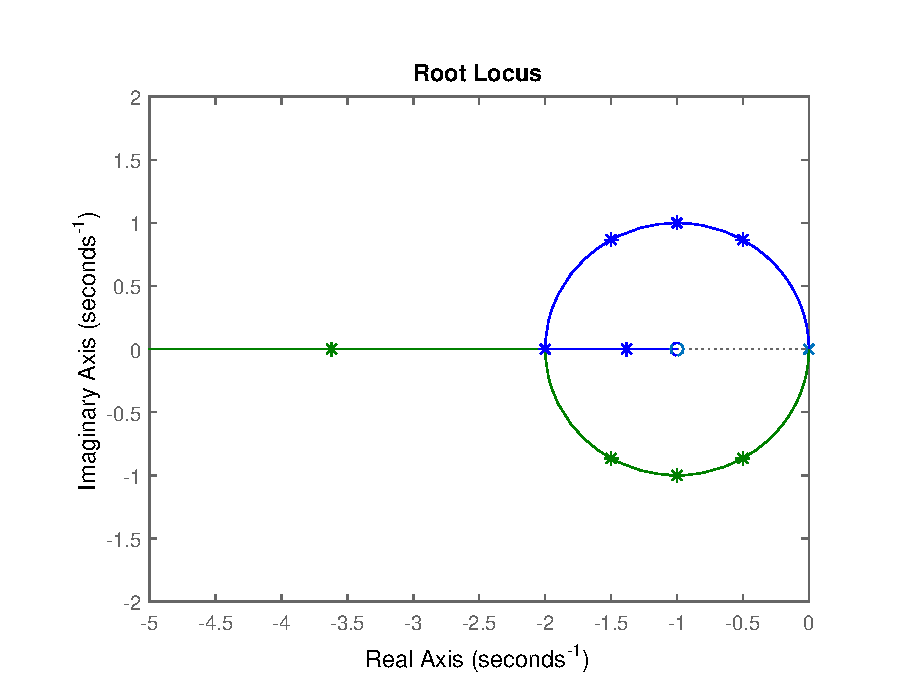
\includegraphics[scale=0.8]{fig1.eps}
		\caption{Matlab plot of the root locus and pole positions for $K \in \{1, 2, 3, 4, 5\}$}
	\end{figure}

%%%%%%%%%%%%%%%%%%%%%%%%%%%%%%%%%%%%%%%%%%%%%%%%%%%%%%%%%%%%%%%%%%%%%%%%%%%%%%%%%%%%%%%%%%%%%%%%%%%%%%%%%%%%%%%%%%%%%%
% Question 3.10 & 3.11
%%%%%%%%%%%%%%%%%%%%%%%%%%%%%%%%%%%%%%%%%%%%%%%%%%%%%%%%%%%%%%%%%%%%%%%%%%%%%%%%%%%%%%%%%%%%%%%%%%%%%%%%%%%%%%%%%%%%%%
	
	\textbf{Question 3.10 \& 3.11}
	
	Code was written to determine the Bode plots and the step responses for the closed loop system for\\ $K \in \{1,2,3,4,5\}$. The code is shown in Appendix B, and the plots can be seen in Figures 6 through 10.
	
	\begin{figure}[h]
		\centering
		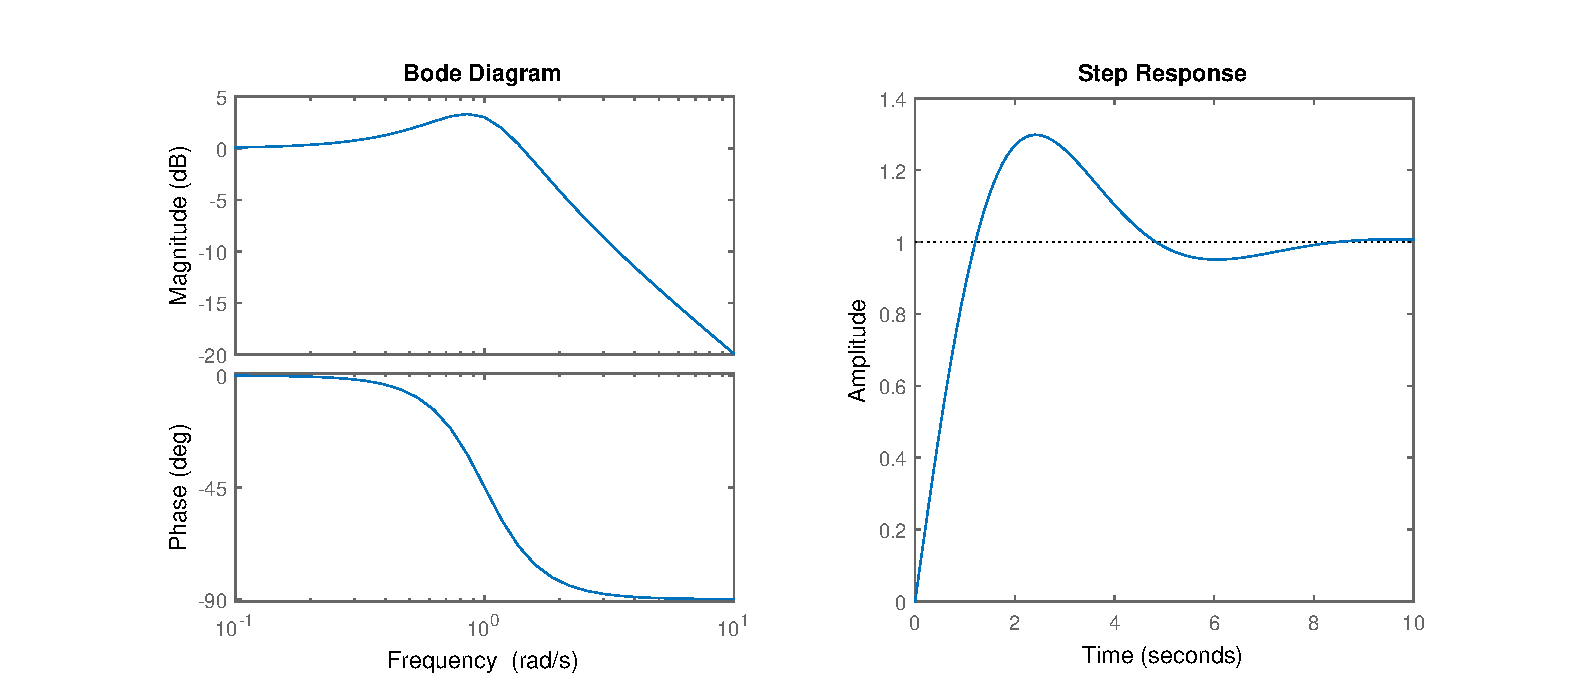
\includegraphics[scale=0.5]{fig2.eps}
		\caption{Closed loop control system with $K = 1$}
	\end{figure}
	
	\begin{figure}[h]
		\centering
		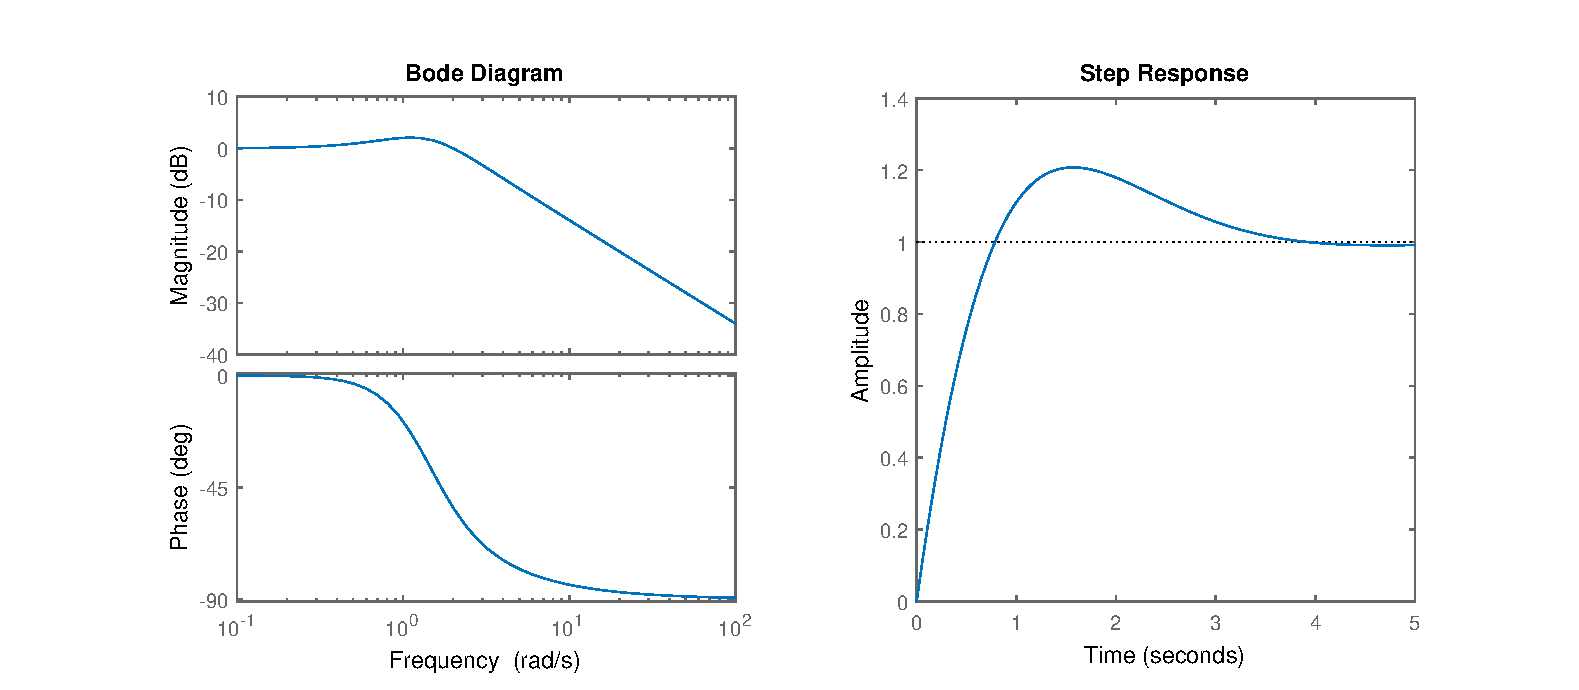
\includegraphics[scale=0.5]{fig3.eps}
		\caption{Closed loop control system with $K = 2$}
	\end{figure}
	
	\begin{figure}[h]
		\centering
		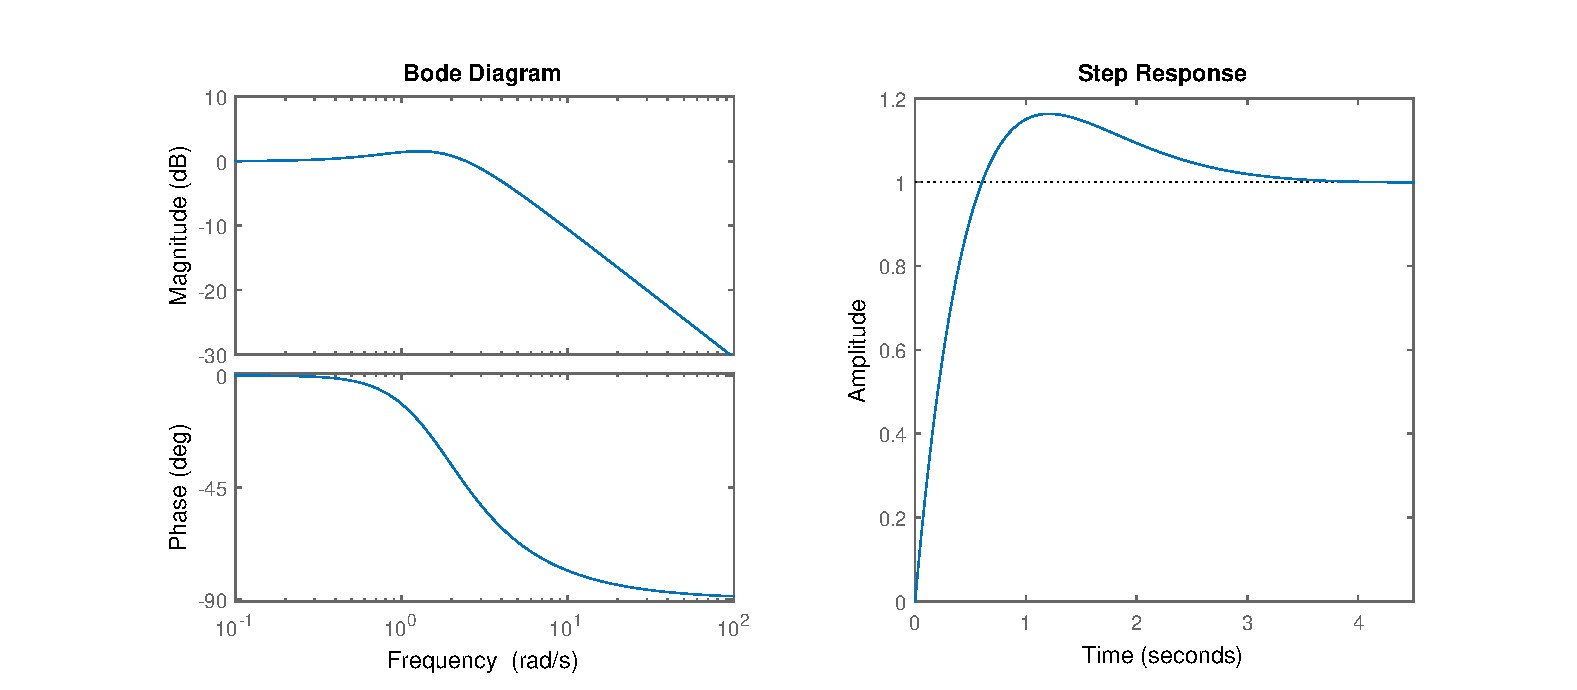
\includegraphics[scale=0.5]{fig4.eps}
		\caption{Closed loop control system with $K = 3$}
	\end{figure}
	
	\begin{figure}[h]
		\centering
		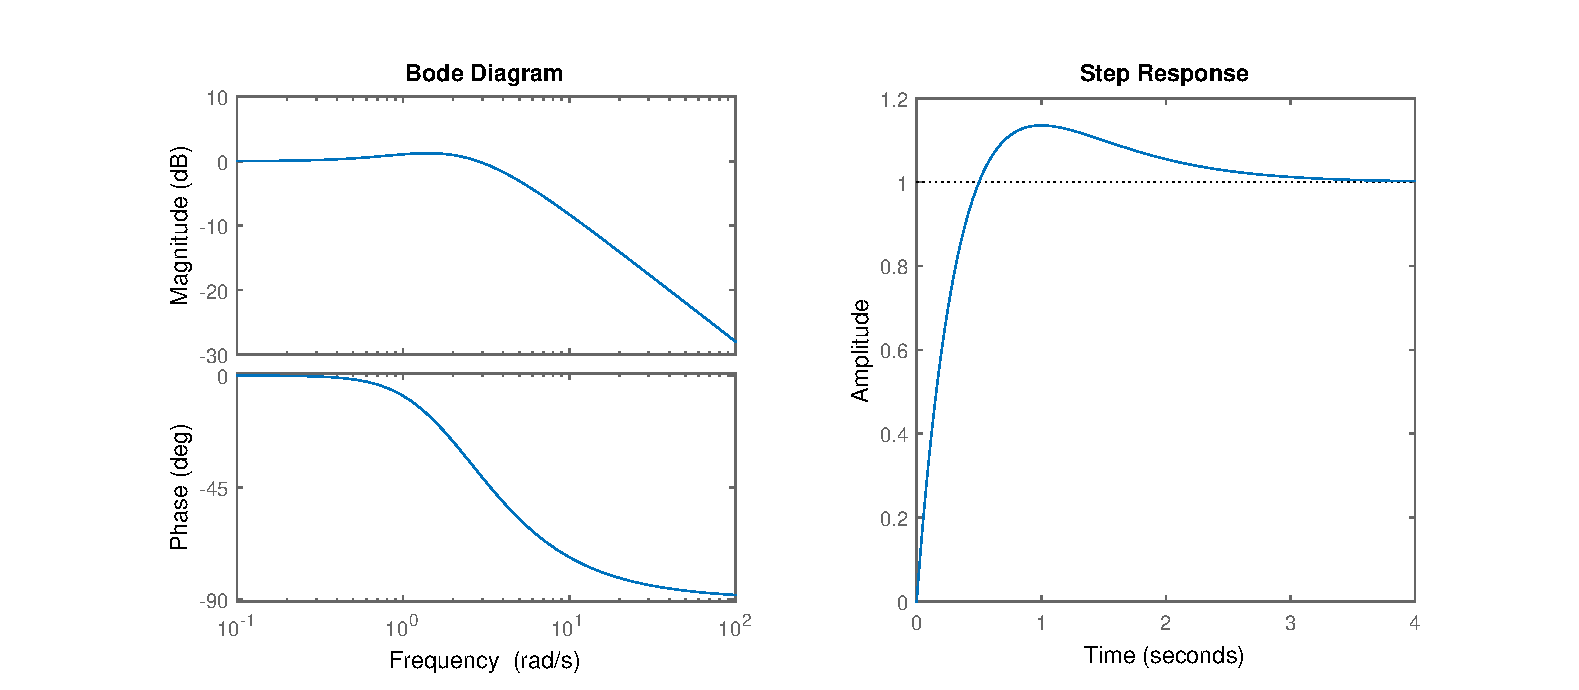
\includegraphics[scale=0.5]{fig5.eps}
		\caption{Closed loop control system with $K = 4$}
	\end{figure}
	
	\begin{figure}[h]
		\centering
		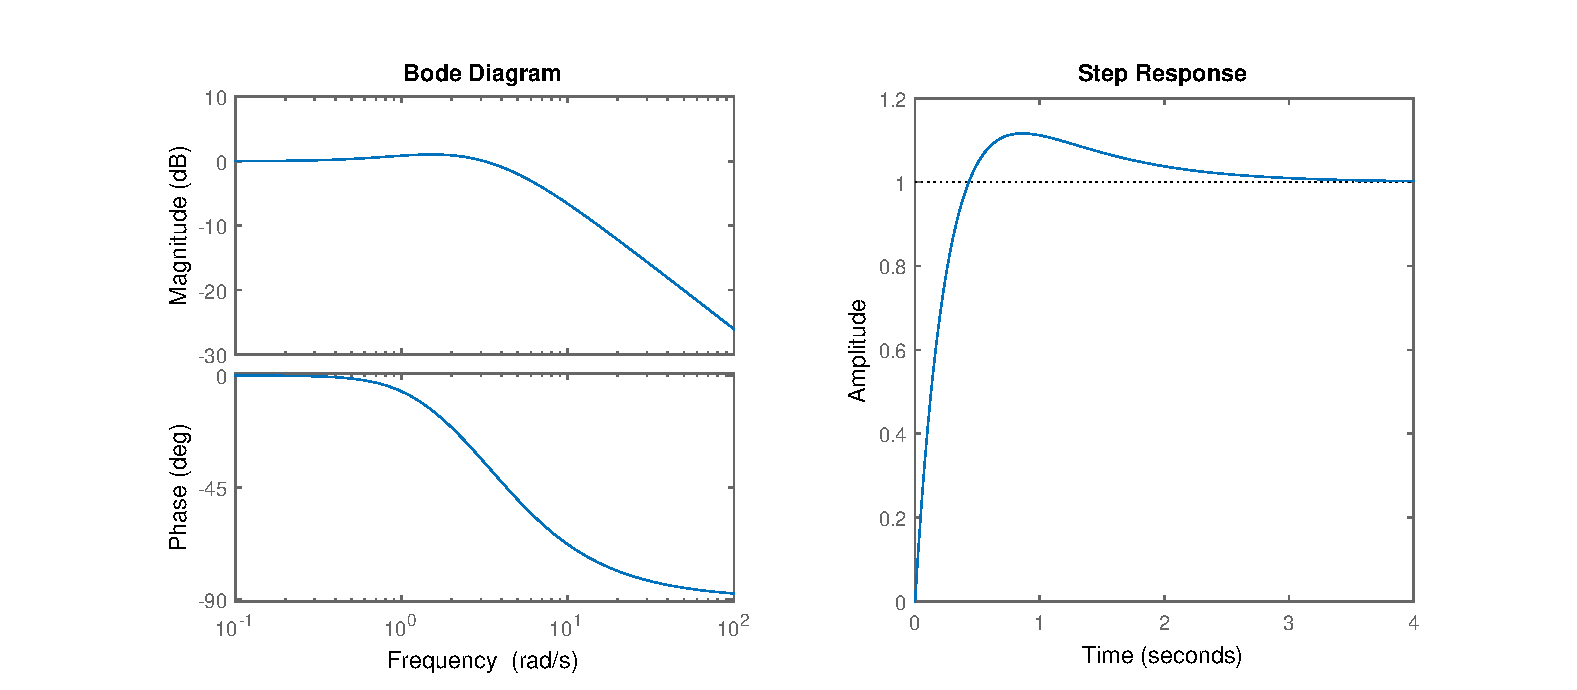
\includegraphics[scale=0.5]{fig6.eps}
		\caption{Closed loop control system with $K = 5$}
	\end{figure}
	
	\newpage
%%%%%%%%%%%%%%%%%%%%%%%%%%%%%%%%%%%%%%%%%%%%%%%%%%%%%%%%%%%%%%%%%%%%%%%%%%%%%%%%%%%%%%%%%%%%%%%%%%%%%%%%%%%%%%%%%%%%%%
% Question 3.12
%%%%%%%%%%%%%%%%%%%%%%%%%%%%%%%%%%%%%%%%%%%%%%%%%%%%%%%%%%%%%%%%%%%%%%%%%%%%%%%%%%%%%%%%%%%%%%%%%%%%%%%%%%%%%%%%%%%%%%
	
	\textbf{Question 3.12}\\
	
	By inspection, we see that the biggest bandwidth occurs when $K = 5$, with $\omega_C \approx 5.93 \si{\radian\per\second}$. Further, we see that when $K = 5$, we get the minimum rise time from our controlled system with the rise time approximately 0.421 seconds. The controller when $K = 5$ has the greatest bandwidth and the smallest rise time. This means that it is the quickest responding controlled system and it is also the system which has the least attenuation of input frequencies. A system that responds quickly is a desirable characteristic. Further, a system that will respond to a wide variety of input signals is also desirable - a large bandwidth will provide for this, however, as the bandwidth of a control system increases, so too does the system's responsiveness to noise or external perturbation. Hence, we want a system with a small rise time, which is not overly responsive to external noise - that is a system with a moderate badnwidth. Finally, we also want a system which does not suffer from overshoot - too much overshoot can damage the controlled system in some instances. A gain of $K = 3$, or $K = 4$ would most likely be a suitable choice between these competing characteristics.
	
	\newpage
%%%%%%%%%%%%%%%%%%%%%%%%%%%%%%%%%%%%%%%%%%%%%%%%%%%%%%%%%%%%%%%%%%%%%%%%%%%%%%%%%%%%%%%%%%%%%%%%%%%%%%%%%%%%%%%%%%%%%%
% Appendix A
%%%%%%%%%%%%%%%%%%%%%%%%%%%%%%%%%%%%%%%%%%%%%%%%%%%%%%%%%%%%%%%%%%%%%%%%%%%%%%%%%%%%%%%%%%%%%%%%%%%%%%%%%%%%%%%%%%%%%%
	
	\textbf{Appendix A}\\
	
	\begin{lstlisting}
		% Clear the workspace and variables
		clear; clc; clf;
		
		% Define the open loop system
		sys = tf([1 1],[1 0 0]);
		
		% Plot the root locus for the open loop system
		rlocus(sys)
		axis([-5 0 -2 2])
		hold on
		
		% Plot the pole locations for various values of the gain
		K = [1 2 3 4 5];
		rlocus(sys,K,'*')
	\end{lstlisting}
	
	\newpage
%%%%%%%%%%%%%%%%%%%%%%%%%%%%%%%%%%%%%%%%%%%%%%%%%%%%%%%%%%%%%%%%%%%%%%%%%%%%%%%%%%%%%%%%%%%%%%%%%%%%%%%%%%%%%%%%%%%%%%
% Appendix B
%%%%%%%%%%%%%%%%%%%%%%%%%%%%%%%%%%%%%%%%%%%%%%%%%%%%%%%%%%%%%%%%%%%%%%%%%%%%%%%%%%%%%%%%%%%%%%%%%%%%%%%%%%%%%%%%%%%%%%

	\textbf{Appendix B}\\
	
	\begin{lstlisting}
		% Clear the workspace and any variables
		clear; clc; clf;
		
		for K = 1:5
			% Define closed loop system
			sys = tf([K K],[1 K K]);
		
			% Create new figure
			figure(K)
		
			% Plot Bode plot for system
			subplot(1,2,1)
			bode(sys)
		
			% Plot Step response for system
			subplot(1,2,2)
			step(sys)
		end
	\end{lstlisting}
	
\end{document}
